
\section{AECM tests for BOS and GOD distributions}
\label{appendix:metrics_synth}

\begin{table}[H]
\centering
\begin{minipage}{.48\columnwidth}
\centering
\begin{adjustbox}{width=\columnwidth}
\begin{tabular}{lllllrrr}
\toprule
 &  &  &  &  & $\Delta \alpha$ & $\Delta \mu$ & $\Delta \pi$ \\
Init. & $n$ & $n_{clusters}$ & $d$ & $n_{cats}$ &  &  &  \\
\midrule
\multirow[t]{16}{*}{K-Means} & \multirow[t]{8}{*}{50} & \multirow[t]{4}{*}{3} & \multirow[t]{2}{*}{3} & 2 & 0.143 & 0.167 & 0.295 \\
 &  &  &  & 3 & 0.135 & 0.667 & 0.116 \\
\cline{4-8}
 &  &  & \multirow[t]{2}{*}{5} & 2 & 0.090 & 0.200 & 0.172 \\
 &  &  &  & 3 & 0.083 & 0.333 & 0.105 \\
\cline{3-8} \cline{4-8}
 &  & \multirow[t]{4}{*}{5} & \multirow[t]{2}{*}{3} & 2 & 0.099 & 0.667 & 0.337 \\
 &  &  &  & 3 & 0.142 & 0.778 & 0.356 \\
\cline{4-8}
 &  &  & \multirow[t]{2}{*}{5} & 2 & 0.099 & 0.400 & 0.210 \\
 &  &  &  & 3 & 0.125 & 0.400 & 0.157 \\
\cline{2-8} \cline{3-8} \cline{4-8}
 & \multirow[t]{8}{*}{250} & \multirow[t]{4}{*}{3} & \multirow[t]{2}{*}{3} & 2 & 0.111 & 0.167 & 0.344 \\
 &  &  &  & 3 & 0.021 & 0.444 & 0.206 \\
\cline{4-8}
 &  &  & \multirow[t]{2}{*}{5} & 2 & 0.152 & 0.200 & 0.162 \\
 &  &  &  & 3 & 0.043 & 0.267 & 0.106 \\
\cline{3-8} \cline{4-8}
 &  & \multirow[t]{4}{*}{5} & \multirow[t]{2}{*}{3} & 2 & 0.149 & 0.667 & 0.423 \\
 &  &  &  & 3 & 0.315 & 0.444 & 0.246 \\
\cline{4-8}
 &  &  & \multirow[t]{2}{*}{5} & 2 & 0.134 & 0.400 & 0.290 \\
 &  &  &  & 3 & 0.174 & 0.467 & 0.129 \\
\cline{1-8} \cline{2-8} \cline{3-8} \cline{4-8}
\multirow[t]{16}{*}{Random} & \multirow[t]{8}{*}{50} & \multirow[t]{4}{*}{3} & \multirow[t]{2}{*}{3} & 2 & 0.112 & 0.167 & 0.074 \\
 &  &  &  & 3 & 0.085 & 0.222 & 0.025 \\
\cline{4-8}
 &  &  & \multirow[t]{2}{*}{5} & 2 & 0.011 & 0.000 & 0.043 \\
 &  &  &  & 3 & 0.039 & 0.067 & 0.038 \\
\cline{3-8} \cline{4-8}
 &  & \multirow[t]{4}{*}{5} & \multirow[t]{2}{*}{3} & 2 & 0.058 & 0.167 & 0.081 \\
 &  &  &  & 3 & 0.073 & 0.111 & 0.079 \\
\cline{4-8}
 &  &  & \multirow[t]{2}{*}{5} & 2 & 0.095 & 0.300 & 0.130 \\
 &  &  &  & 3 & 0.068 & 0.067 & 0.117 \\
\cline{2-8} \cline{3-8} \cline{4-8}
 & \multirow[t]{8}{*}{250} & \multirow[t]{4}{*}{3} & \multirow[t]{2}{*}{3} & 2 & 0.095 & 0.000 & 0.035 \\
 &  &  &  & 3 & 0.018 & 0.222 & 0.007 \\
\cline{4-8}
 &  &  & \multirow[t]{2}{*}{5} & 2 & 0.031 & 0.000 & 0.016 \\
 &  &  &  & 3 & 0.017 & 0.067 & 0.019 \\
\cline{3-8} \cline{4-8}
 &  & \multirow[t]{4}{*}{5} & \multirow[t]{2}{*}{3} & 2 & 0.037 & 0.167 & 0.022 \\
 &  &  &  & 3 & 0.057 & 0.222 & 0.037 \\
\cline{4-8}
 &  &  & \multirow[t]{2}{*}{5} & 2 & 0.044 & 0.000 & 0.022 \\
 &  &  &  & 3 & 0.020 & 0.067 & 0.052 \\
\cline{1-8} \cline{2-8} \cline{3-8} \cline{4-8}
\bottomrule
\end{tabular}
\end{adjustbox}
\caption{Results of the experiments for the AECM algorithm no synthetic data with the BOS distribution. The parameters are the number of samples $n$, the number of clusters $n_{clusters}$, the dimension $d$ and the number of categories $n_{cats}$. The deltas are the average of the $L_1$ distances between the true and estimated parameters after applying optimal transport to find the correct clusters.}
\label{tab:results_bos}
\end{minipage} \hspace{.02\columnwidth}%
\begin{minipage}{.48\columnwidth}
\centering
\begin{adjustbox}{width=\columnwidth}
\begin{tabular}{lllllrrr}
\toprule
 &  &  &  &  & $\Delta \alpha$ & $\Delta \mu$ & $\Delta \pi$ \\
Init. & $n$ & $n_{clusters}$ & $d$ & $n_{cats}$ &  &  &  \\
\midrule
\multirow[t]{16}{*}{K-Means} & \multirow[t]{8}{*}{50} & \multirow[t]{4}{*}{3} & \multirow[t]{2}{*}{3} & 2 & 0.103 & 0.167 & 0.166 \\
 &  &  &  & 3 & 0.132 & 0.444 & 0.095 \\
\cline{4-8}
 &  &  & \multirow[t]{2}{*}{5} & 2 & 0.063 & 0.300 & 0.088 \\
 &  &  &  & 3 & 0.074 & 0.067 & 0.020 \\
\cline{3-8} \cline{4-8}
 &  & \multirow[t]{4}{*}{5} & \multirow[t]{2}{*}{3} & 2 & 0.082 & 0.333 & 0.207 \\
 &  &  &  & 3 & 0.149 & 0.778 & 0.118 \\
\cline{4-8}
 &  &  & \multirow[t]{2}{*}{5} & 2 & 0.102 & 0.300 & 0.122 \\
 &  &  &  & 3 & 0.194 & 0.400 & 0.089 \\
\cline{2-8} \cline{3-8} \cline{4-8}
 & \multirow[t]{8}{*}{250} & \multirow[t]{4}{*}{3} & \multirow[t]{2}{*}{3} & 2 & 0.093 & 0.167 & 0.152 \\
 &  &  &  & 3 & 0.079 & 0.222 & 0.076 \\
\cline{4-8}
 &  &  & \multirow[t]{2}{*}{5} & 2 & 0.088 & 0.200 & 0.071 \\
 &  &  &  & 3 & 0.121 & 0.267 & 0.073 \\
\cline{3-8} \cline{4-8}
 &  & \multirow[t]{4}{*}{5} & \multirow[t]{2}{*}{3} & 2 & 0.083 & 0.833 & 0.211 \\
 &  &  &  & 3 & 0.104 & 0.889 & 0.125 \\
\cline{4-8}
 &  &  & \multirow[t]{2}{*}{5} & 2 & 0.097 & 0.300 & 0.110 \\
 &  &  &  & 3 & 0.113 & 0.400 & 0.064 \\
\cline{1-8} \cline{2-8} \cline{3-8} \cline{4-8}
\multirow[t]{16}{*}{Random} & \multirow[t]{8}{*}{50} & \multirow[t]{4}{*}{3} & \multirow[t]{2}{*}{3} & 2 & 0.063 & 0.167 & 0.104 \\
 &  &  &  & 3 & 0.113 & 0.333 & 0.084 \\
\cline{4-8}
 &  &  & \multirow[t]{2}{*}{5} & 2 & 0.050 & 0.100 & 0.057 \\
 &  &  &  & 3 & 0.075 & 0.267 & 0.053 \\
\cline{3-8} \cline{4-8}
 &  & \multirow[t]{4}{*}{5} & \multirow[t]{2}{*}{3} & 2 & 0.058 & 0.333 & 0.145 \\
 &  &  &  & 3 & 0.177 & 0.667 & 0.092 \\
\cline{4-8}
 &  &  & \multirow[t]{2}{*}{5} & 2 & 0.083 & 0.400 & 0.112 \\
 &  &  &  & 3 & 0.153 & 0.467 & 0.056 \\
\cline{2-8} \cline{3-8} \cline{4-8}
 & \multirow[t]{8}{*}{250} & \multirow[t]{4}{*}{3} & \multirow[t]{2}{*}{3} & 2 & 0.032 & 0.167 & 0.093 \\
 &  &  &  & 3 & 0.197 & 0.222 & 0.042 \\
\cline{4-8}
 &  &  & \multirow[t]{2}{*}{5} & 2 & 0.014 & 0.200 & 0.050 \\
 &  &  &  & 3 & 0.072 & 0.133 & 0.017 \\
\cline{3-8} \cline{4-8}
 &  & \multirow[t]{4}{*}{5} & \multirow[t]{2}{*}{3} & 2 & 0.052 & 0.167 & 0.118 \\
 &  &  &  & 3 & 0.098 & 0.889 & 0.146 \\
\cline{4-8}
 &  &  & \multirow[t]{2}{*}{5} & 2 & 0.058 & 0.400 & 0.085 \\
 &  &  &  & 3 & 0.164 & 0.400 & 0.046 \\
\cline{1-8} \cline{2-8} \cline{3-8} \cline{4-8}
\bottomrule
\end{tabular}
\end{adjustbox}
\caption{Results of the experiments for the AECM algorithm no synthetic data with the GOD model. The parameters are the number of samples $n$, the number of clusters $n_{clusters}$, the dimension $d$ and the number of categories $n_{cats}$. The deltas are the average of the $L_1$ distances between the true and estimated parameters after applying optimal transport to find the correct clusters.}
\label{tab:results_god}
\end{minipage}
\end{table}

\section{Metrics on real-world datasets}
\label{appendix:metrics_real}

\begin{figure}[H]
    \centering
    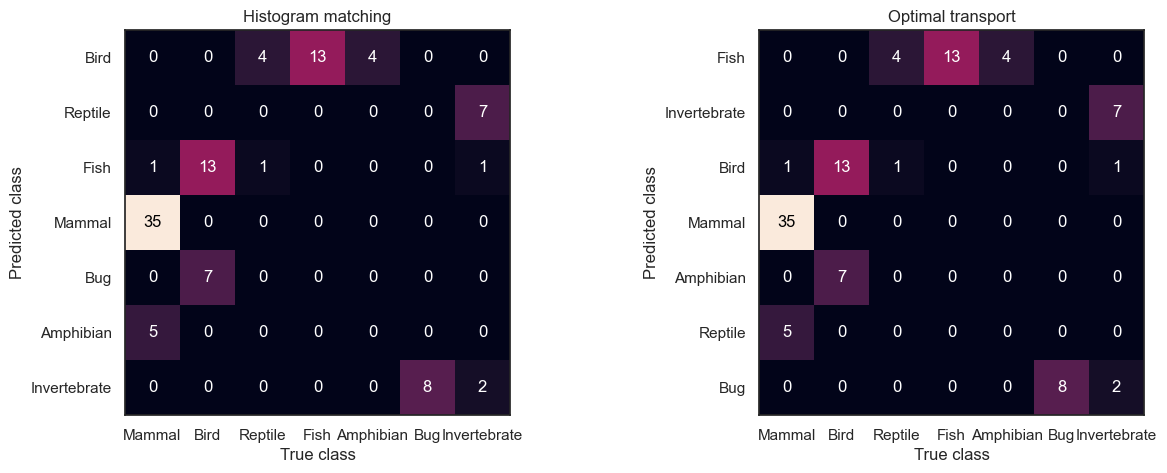
\includegraphics[width=\textwidth]{Attachments/assignment_method.png}
    \caption{Illustration of the two assignment matrices from the different methods after clustering the Zoo dataset. On the left, the naive method and on the right, the optimal assignment method.
    The numbers in the matrices represent the number of samples in the predicted cluster $i$ that are in the true cluster $j$.}
    \label{fig:assignment_methods}
\end{figure}

\begin{table}
\begin{adjustbox}{width=\columnwidth}
\begin{tabular}{lllllll}
\toprule
 &  & \textbf{Runtime (s)} & \textbf{F1} & \textbf{Accuracy} & \textbf{Wasserstein} & \textbf{ARI} \\
Dataset & Method &  &  &  &  &  \\
\midrule
\multirow[t]{6}{*}{\textbf{Zoo}} & \textbf{BOS Random} & 47.28 & 0.77 & 0.78 & 0.35 & \textbf{\underline{0.76}} \\
\textbf{} & \textbf{BOS K-Means} & 4.75 & \textbf{\underline{0.86}} & \textbf{\underline{0.84}} & 0.17 & 0.90 \\
\textbf{} & \textbf{GOD Random} & 52.64 & 0.87 & 0.86 & 0.23 & 0.83 \\
\textbf{} & \textbf{GOD K-Means} & 15.12 & 0.87 & 0.85 & \textbf{\underline{0.14}} & 0.90 \\
\textbf{} & \textbf{K-Means} & \textbf{\underline{0.01}} & 0.70 & 0.64 & 0.84 & 0.58 \\
\textbf{} & \textbf{Gaussian} & 0.75 & 0.79 & 0.76 & 0.33 & 0.73 \\
\cline{1-7}
\multirow[t]{6}{*}{\textbf{Car Evaluation}} & \textbf{BOS Random} & 481.93 & 0.46 & 0.40 & 0.66 & 0.02 \\
\textbf{} & \textbf{BOS K-Means} & 415.80 & 0.42 & 0.37 & 0.73 & -0.01 \\
\textbf{} & \textbf{GOD Random} & 28.95 & 0.43 & 0.40 & 0.41 & -0.04 \\
\textbf{} & \textbf{GOD K-Means} & 19.26 & 0.46 & 0.39 & 0.94 & 0.05 \\
\textbf{} & \textbf{K-Means} & \textbf{\underline{0.01}} & 0.41 & 0.34 & 0.91 & 0.01 \\
\textbf{} & \textbf{Gaussian} & 0.04 & 0.44 & 0.36 & 1.07 & 0.02 \\
\cline{1-7}
\multirow[t]{6}{*}{\textbf{Hayes-Roth}} & \textbf{BOS Random} & 307.60 & 0.37 & 0.39 & 0.25 & 0.00 \\
\textbf{} & \textbf{BOS K-Means} & 101.11 & 0.36 & 0.36 & 0.30 & -0.01 \\
\textbf{} & \textbf{GOD Random} & 11.22 & 0.37 & 0.39 & \textbf{\underline{0.25}} & -0.01 \\
\textbf{} & \textbf{GOD K-Means} & 8.49 & 0.37 & 0.36 & 0.23 & -0.01 \\
\textbf{} & \textbf{K-Means} & \textbf{\underline{0.00}} & 0.34 & 0.33 & 0.16 & -0.01 \\
\textbf{} & \textbf{Gaussian} & 0.02 & \textbf{\underline{0.45}} & \textbf{\underline{0.45}} & 0.11 & \textbf{\underline{0.07}} \\
\cline{1-7}
\multirow[t]{6}{*}{\textbf{Caesarian}} & \textbf{BOS Random} & 52.78 & 0.41 & 0.56 & 0.41 & -0.01 \\
\textbf{} & \textbf{BOS K-Means} & 35.48 & 0.53 & 0.53 & 0.05 & -0.01 \\
\textbf{} & \textbf{GOD Random} & 3.47 & 0.54 & 0.54 & \textbf{\underline{0.04}} & -0.01 \\
\textbf{} & \textbf{GOD K-Means} & 3.51 & 0.59 & 0.59 & 0.09 & 0.02 \\
\textbf{} & \textbf{K-Means} & \textbf{\underline{0.01}} & 0.56 & 0.56 & 0.09 & 0.00 \\
\textbf{} & \textbf{Gaussian} & 0.02 & \textbf{\underline{0.60}} & \textbf{\underline{0.60}} & 0.00 & \textbf{\underline{0.03}} \\
\cline{1-7}
\bottomrule
\end{tabular}
\end{adjustbox}
\caption{
Results of the classification task for the different datasets and the proposed methods. 
The metrics are the F1-score, the accuracy, the Wasserstein distance and the adjusted rand index (ARI). 
The runtime is also reported. 
The best results for each dataset and metric are highlighted in bold and underlined. 
}
\label{tab:results_real}
\end{table}
%\tm{Penser à mettre en avant les bons résultats. Eventuellement ajouter les temps de calcul}

\section{t-SNE plots}
\label{sec:appendix_tsne}
\begin{figure}[H]
    \centering
    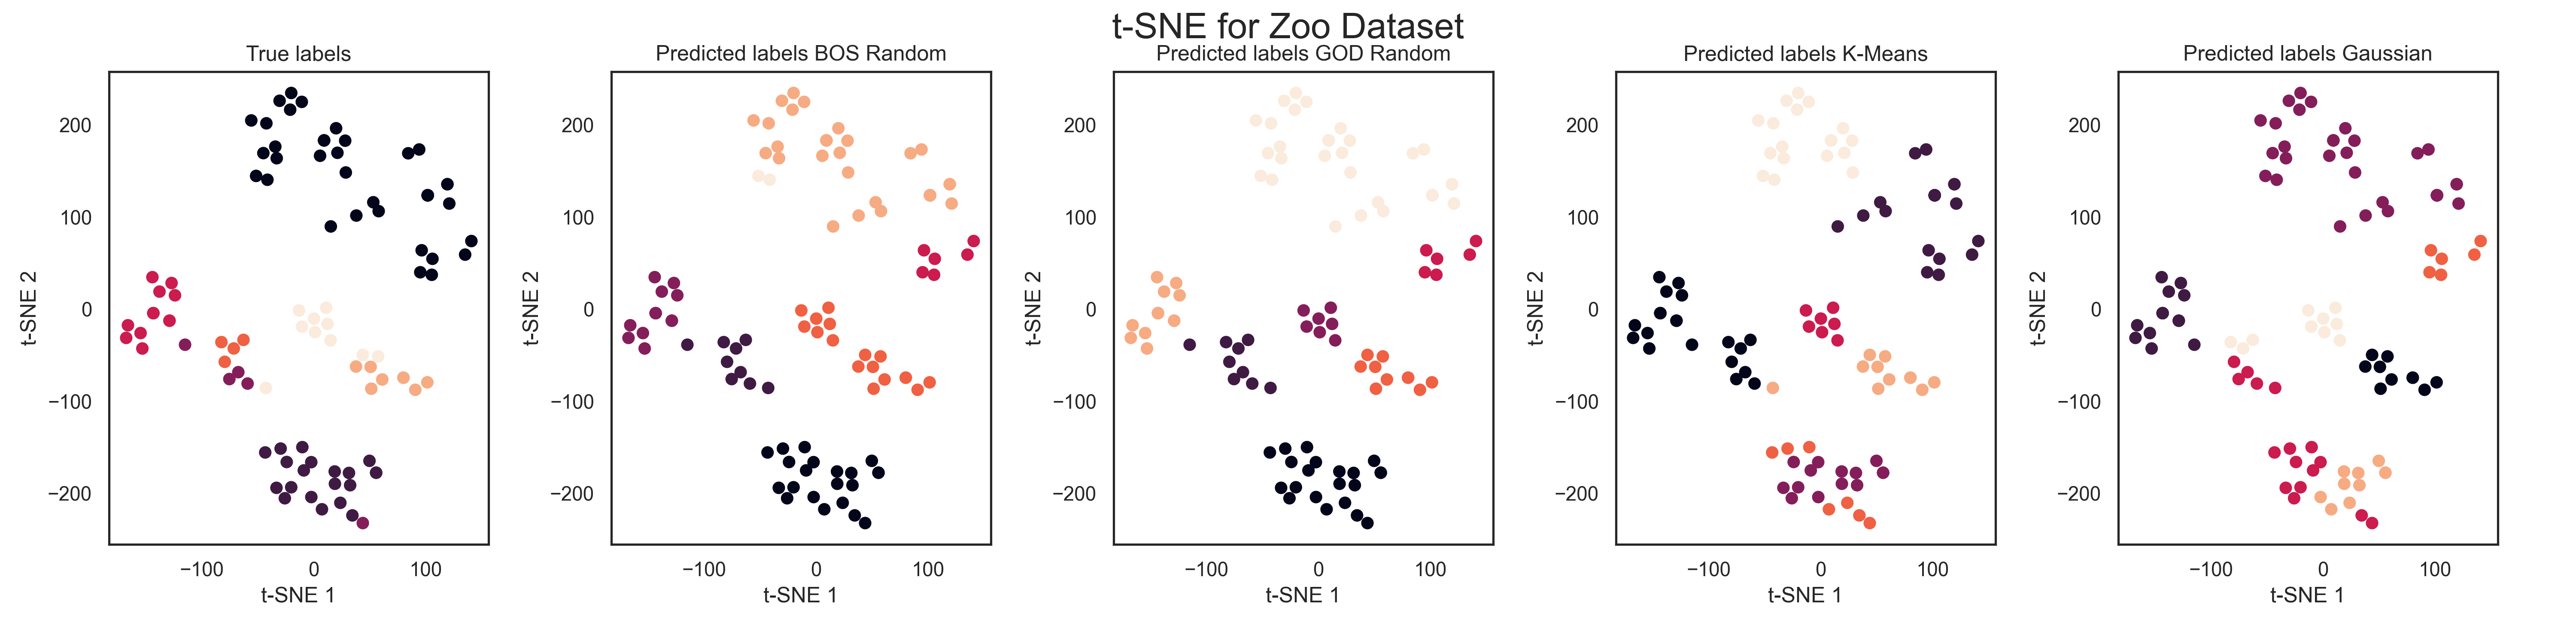
\includegraphics[width=\textwidth]{Attachments/tsne_zoo.png}
    \caption{t-SNE visualization of the Zoo dataset with the true labels and the predicted clusters for the BOS model with random initialization, the GOD model with random initialization, the K-Means algorithm and the Gaussian Mixture Models.}
    \label{fig:tsne_zoo}
\end{figure}

\begin{figure}[H]
    \centering
    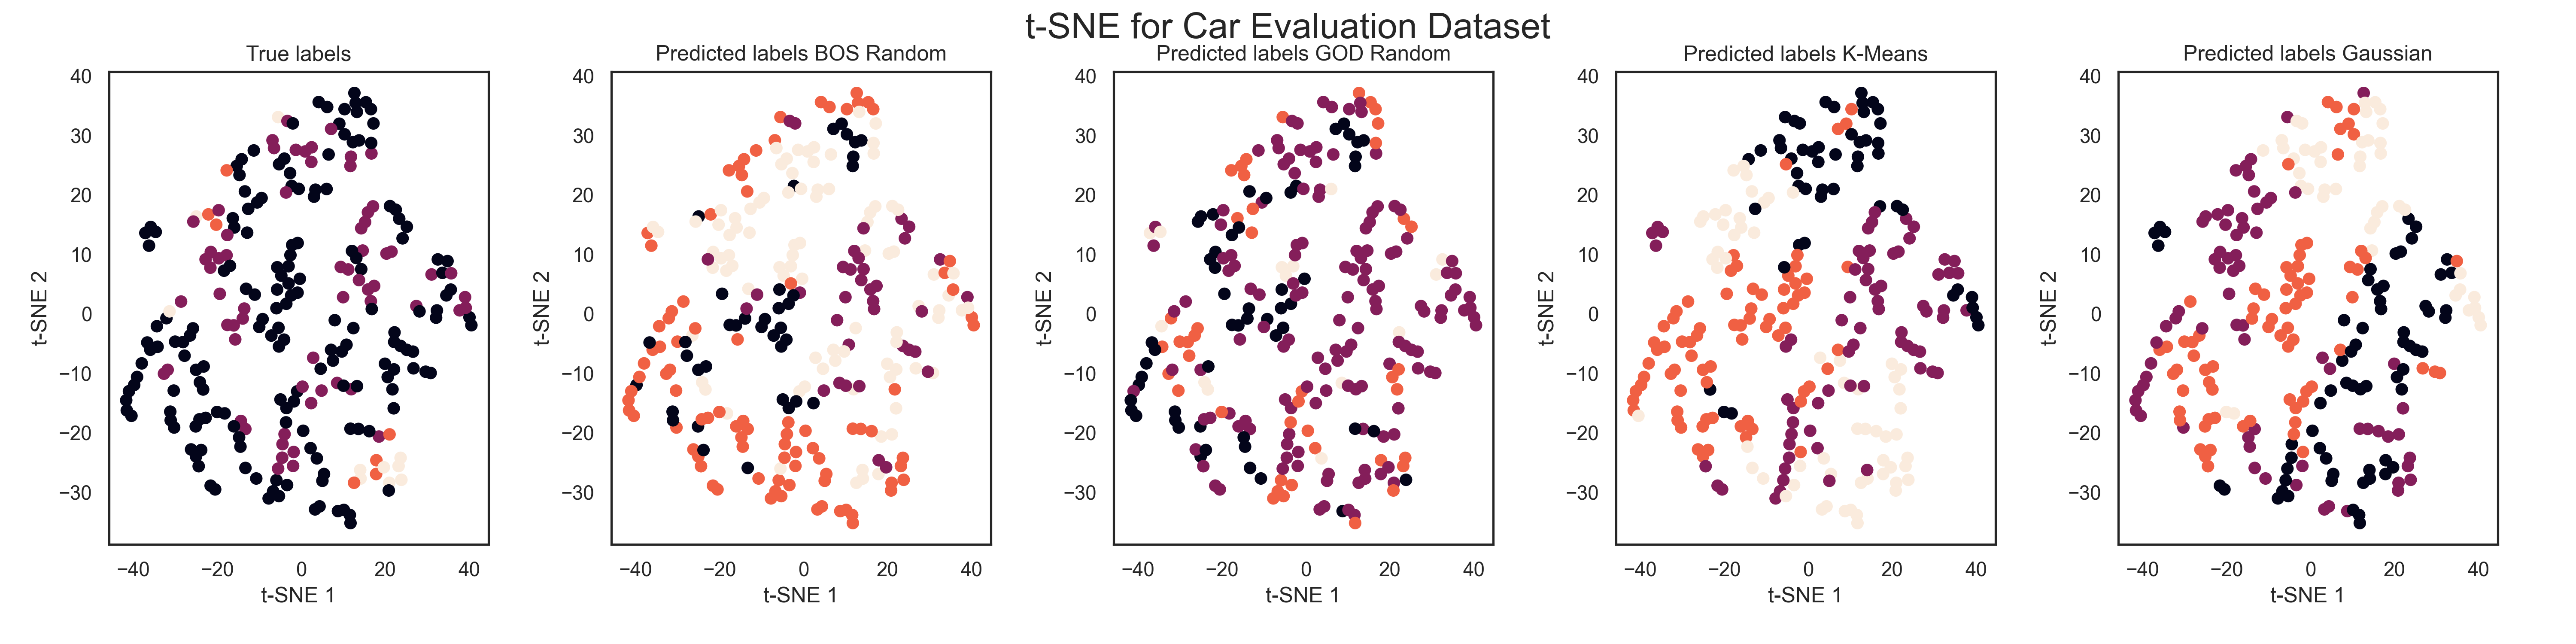
\includegraphics[width=\textwidth]{Attachments/tsne_car_evaluation.png}
    \caption{t-SNE visualization of the Car Evaluation dataset with the true labels and the predicted clusters for the BOS model with random initialization, the GOD model with random initialization, the K-Means algorithm and the Gaussian Mixture Models.}
    \label{fig:tsne_car}
\end{figure}

\begin{figure}[H]
    \centering
    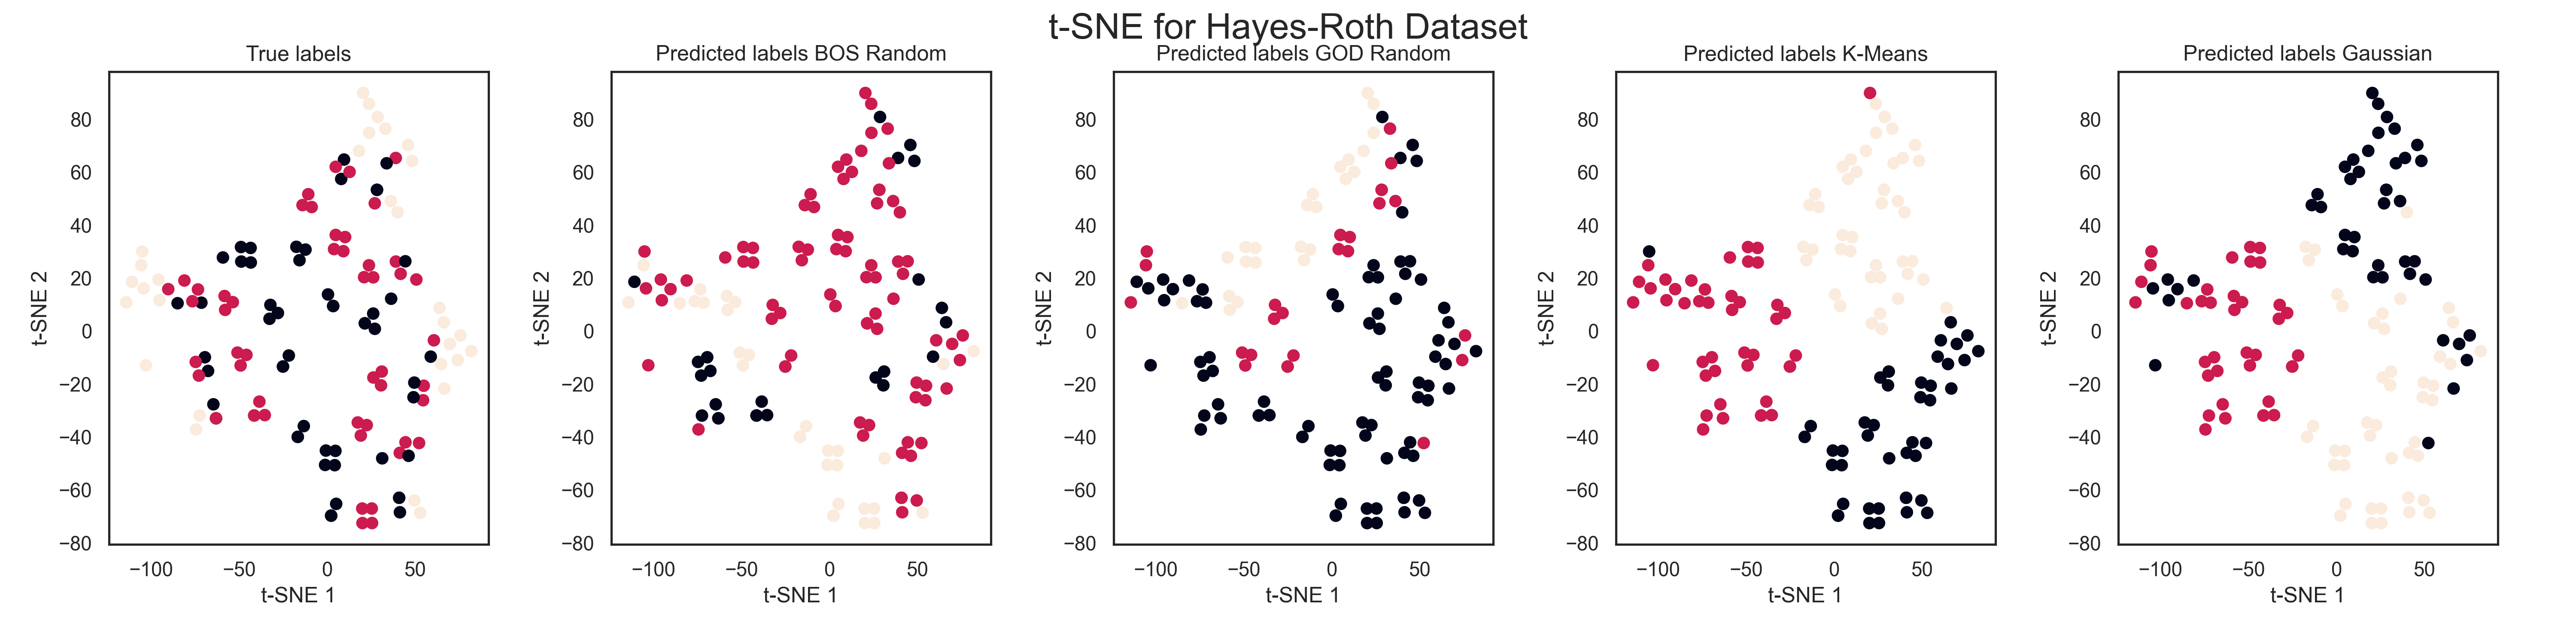
\includegraphics[width=\textwidth]{Attachments/tsne_hayes-roth.png}
    \caption{t-SNE visualization of the Hayes-Roth dataset with the true labels and the predicted clusters for the BOS model with random initialization, the GOD model with random initialization, the K-Means algorithm and the Gaussian Mixture Models.}
    \label{fig:tsne_hr}
\end{figure}

% \begin{figure}[H]
%     \centering
%     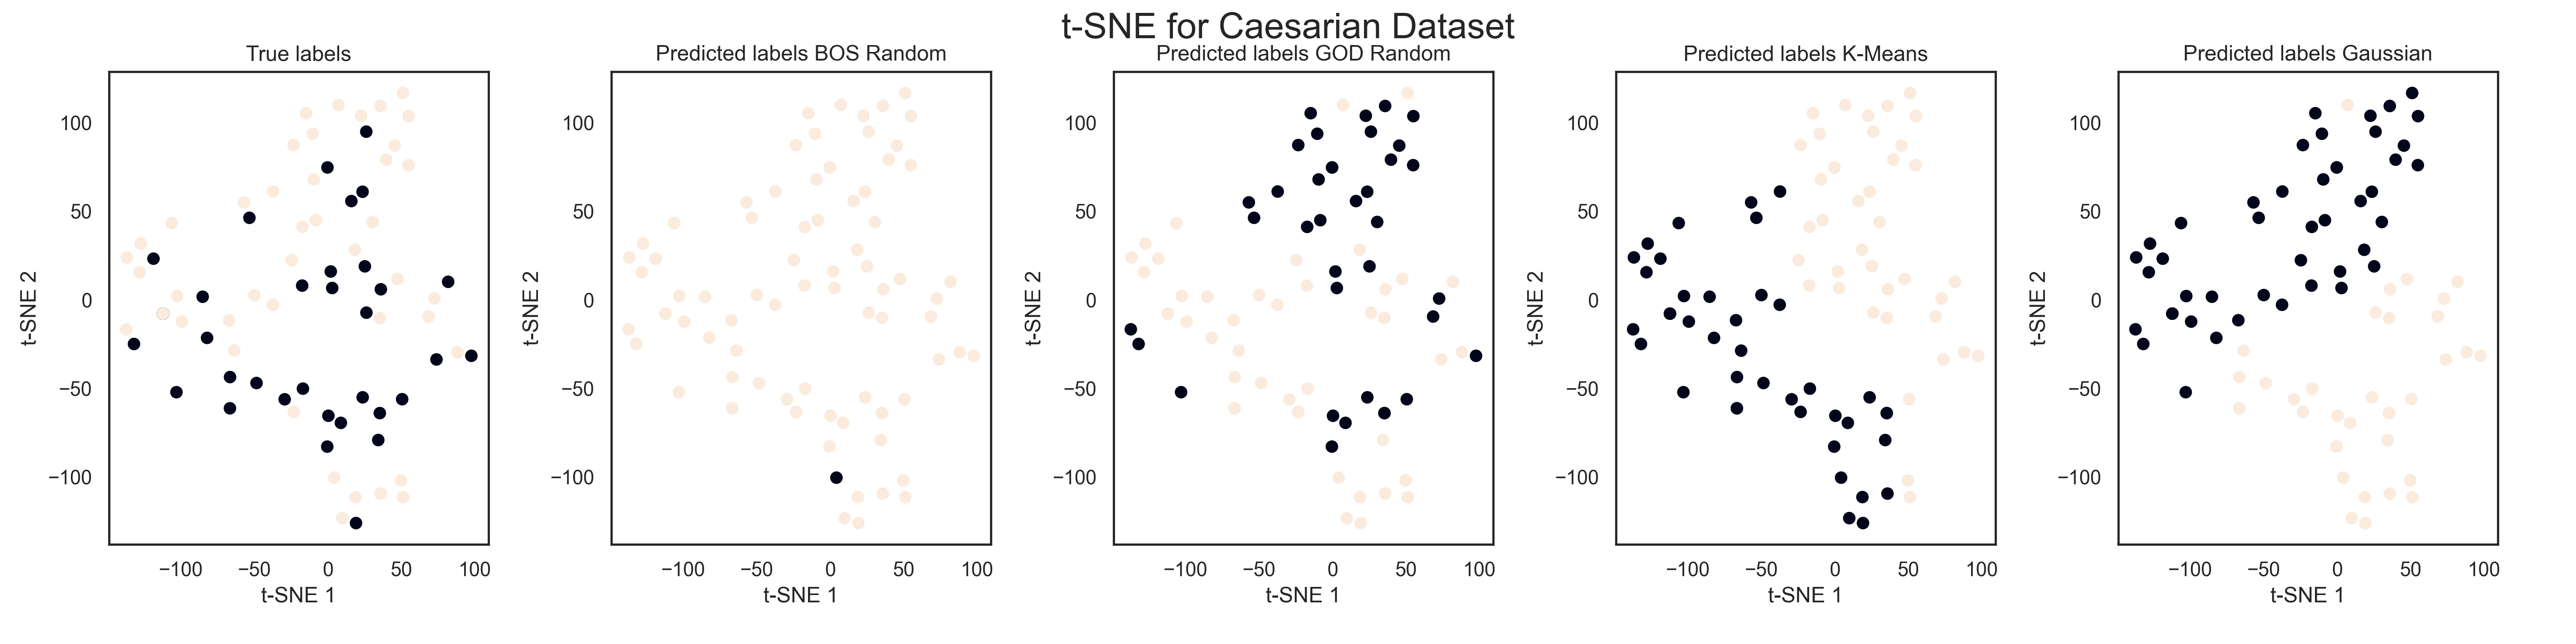
\includegraphics[width=\textwidth]{Attachments/tsne_caesarian.png}
%     \caption{t-SNE visualization of the Caesarian dataset with the true labels and the predicted clusters for the BOS model with random initialization, the GOD model with random initialization, the K-Means algorithm and the Gaussian Mixture Models.}
%     \label{fig:tsne_caesarian}
% \end{figure}

\section{Assignment Matrices}
\label{sec:appendix_assign}

\begin{figure}[H]
    \centering
    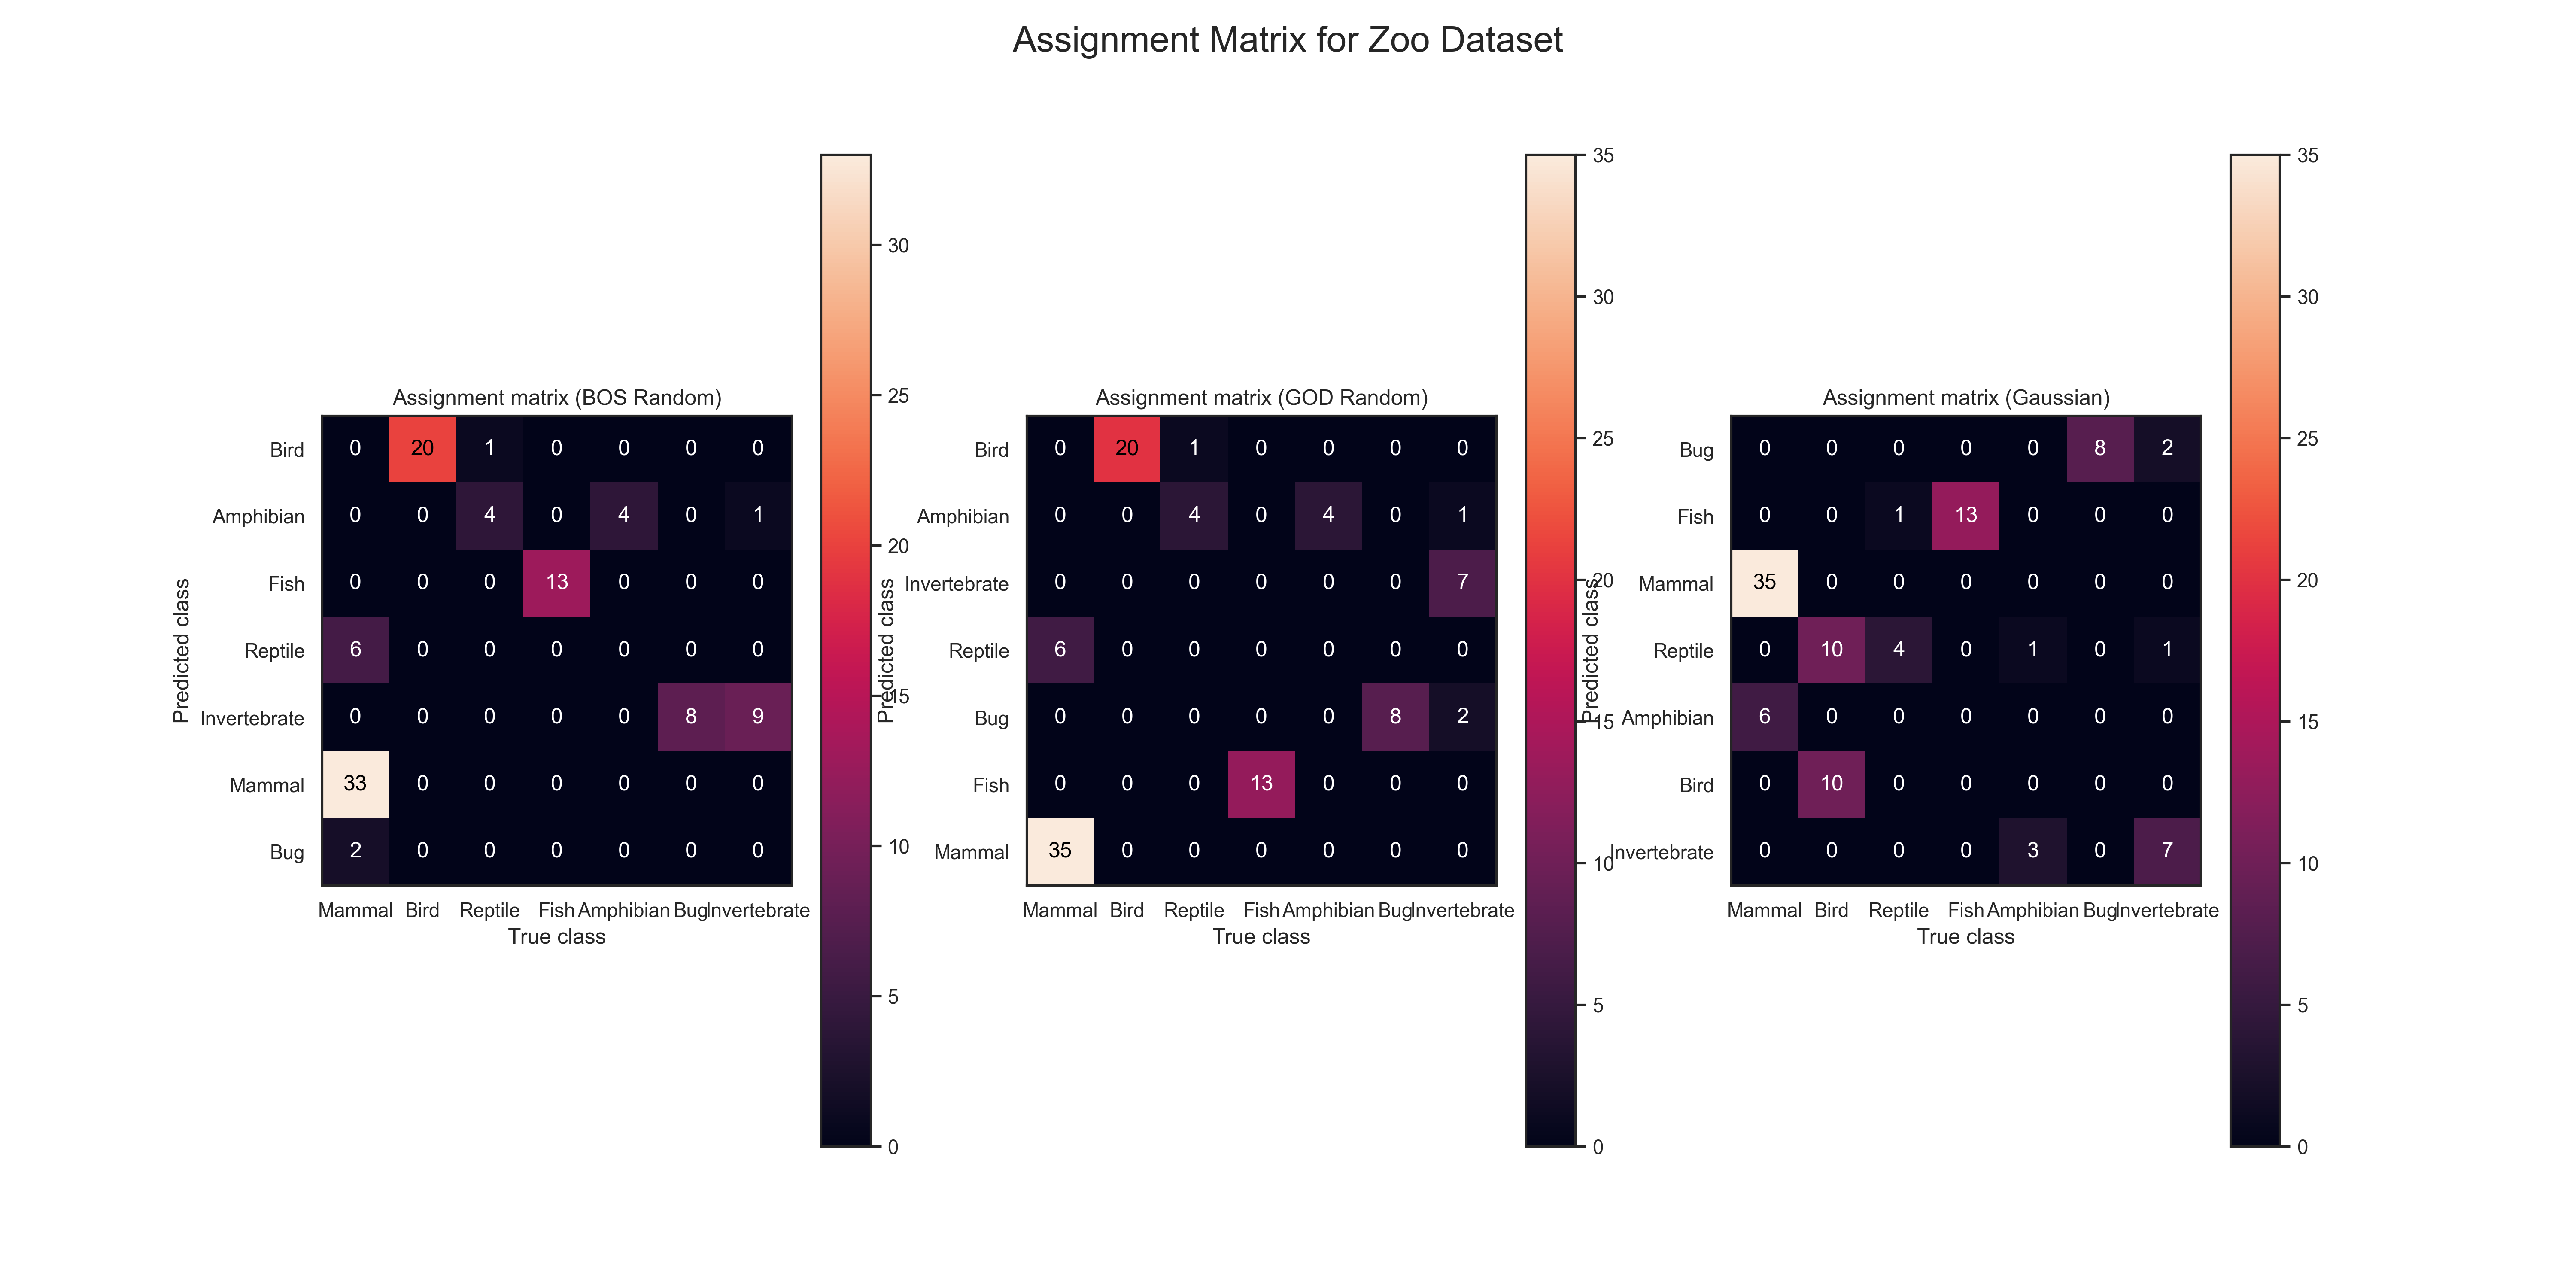
\includegraphics[width=\linewidth]{Attachments/assignment_matrix_zoo.png}
    \caption{Assignment matrix for the Zoo dataset with different methods.}
    \label{fig:assign_zoo}
\end{figure}

\begin{figure}[H]
    \centering
    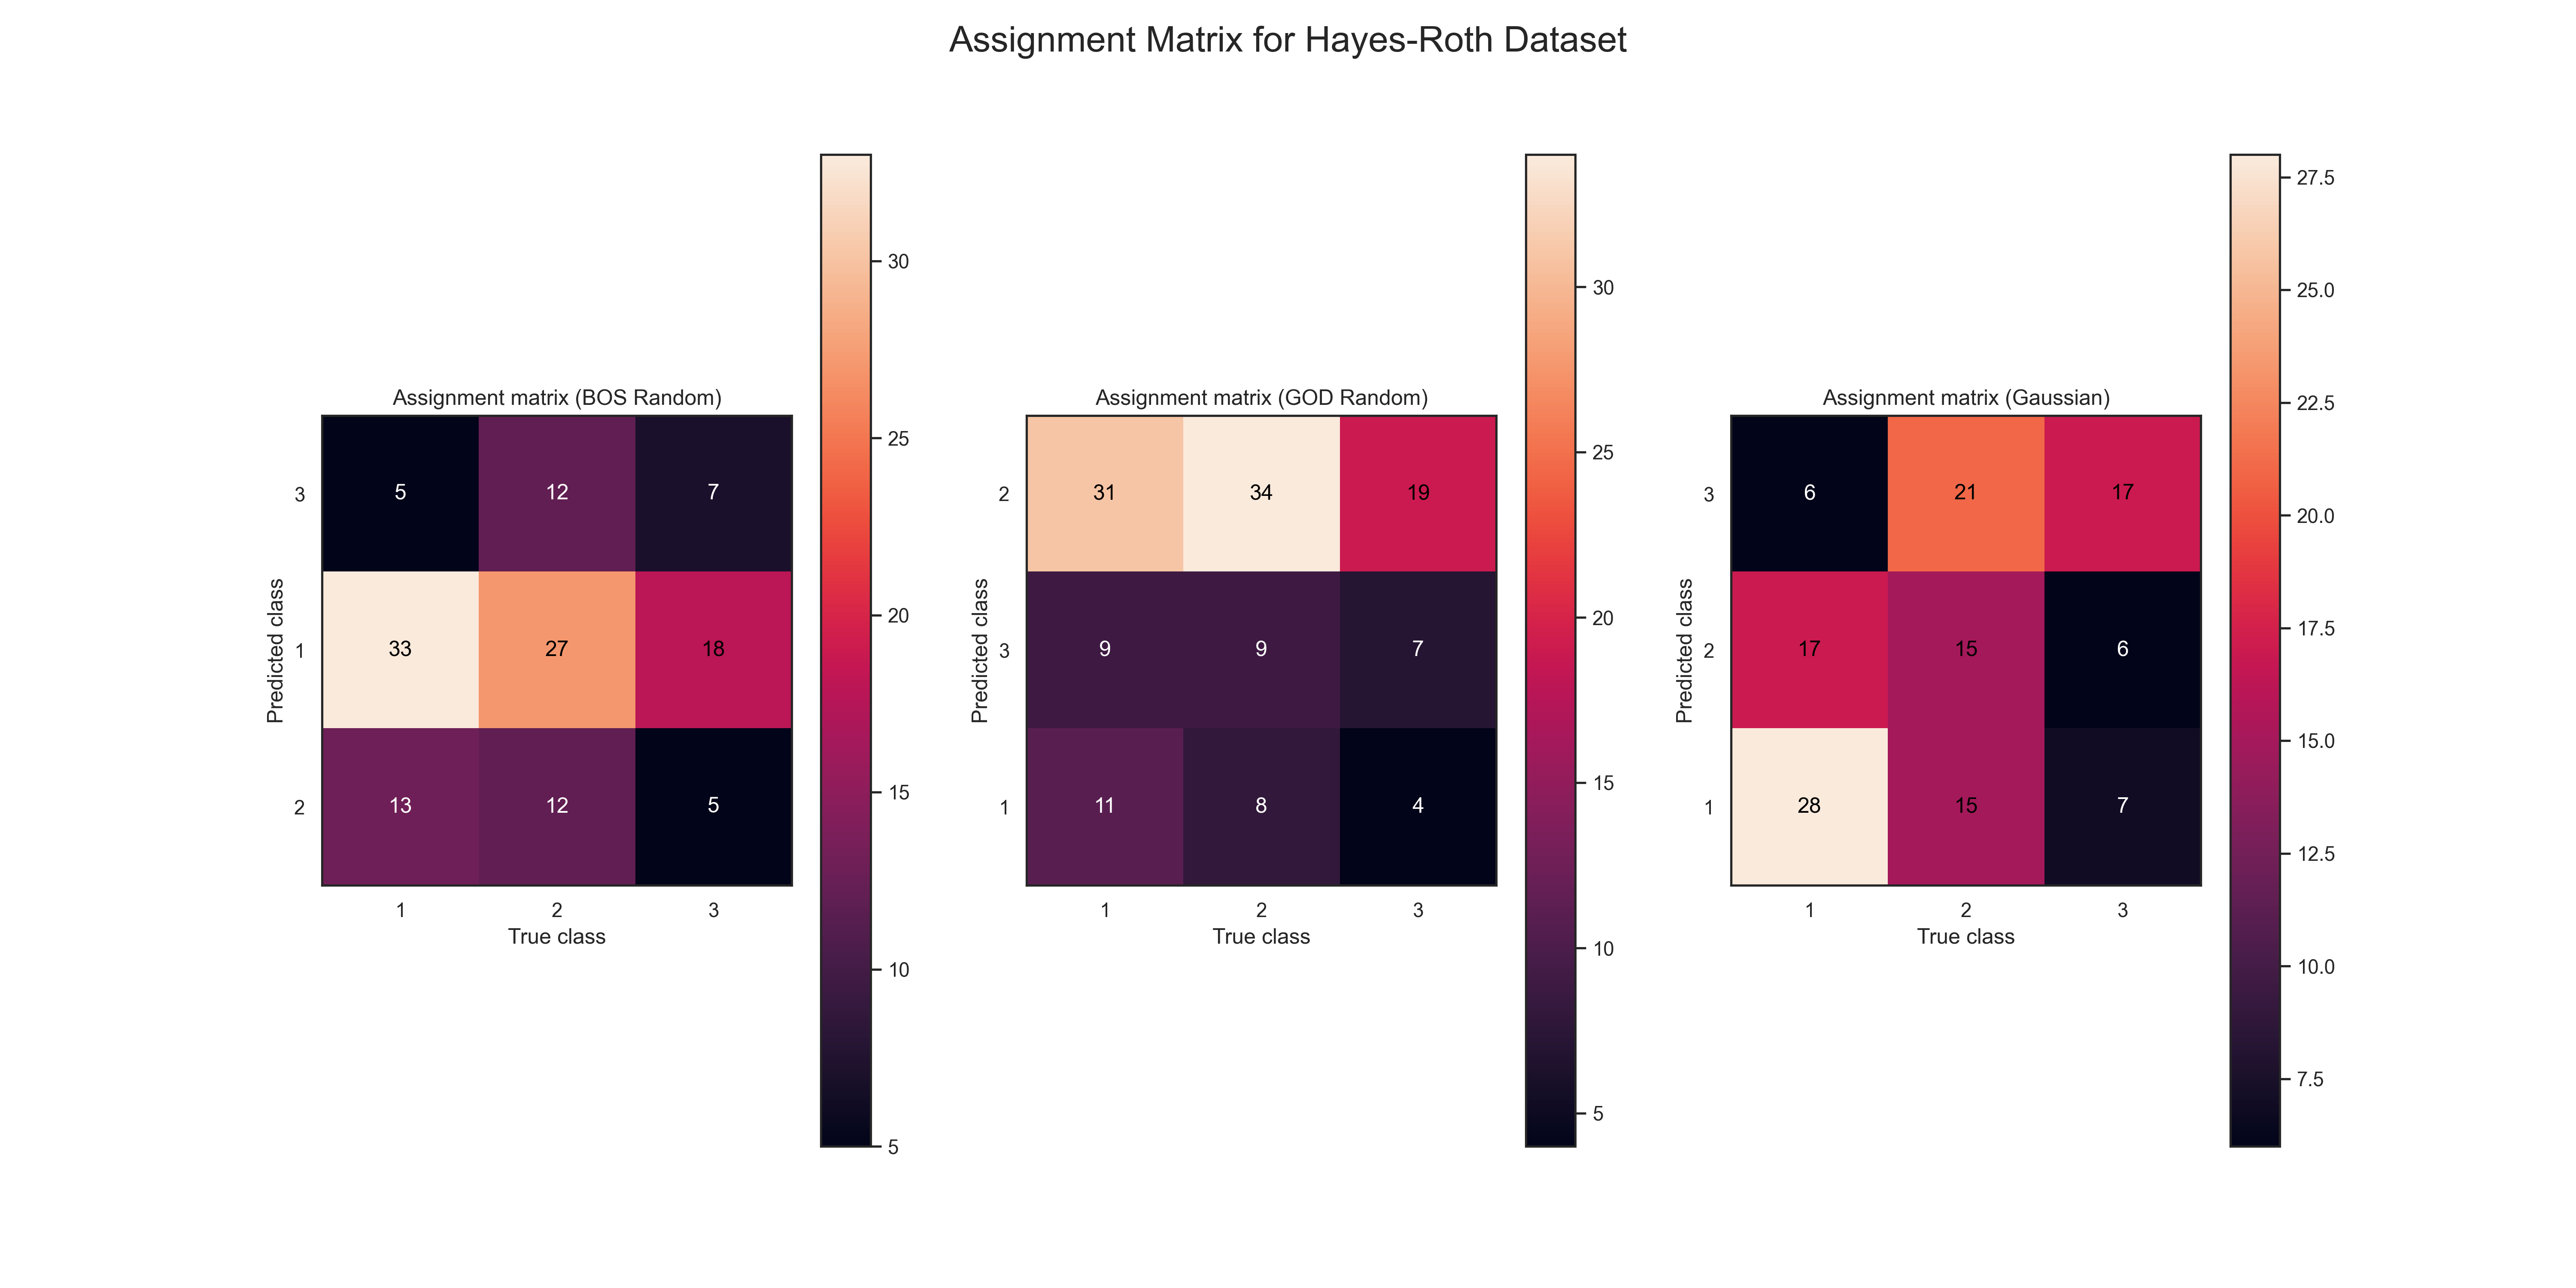
\includegraphics[width=\linewidth]{Attachments/assignment_matrix_hayes-roth.png}
    \caption{Assignment matrix for the Hayes-Roth dataset with different methods.}
    \label{fig:assign_hr}
\end{figure}

\section{Histograms of the different clustering}
\label{sec:appendix_hist}

\begin{figure}[H]
    \centering
    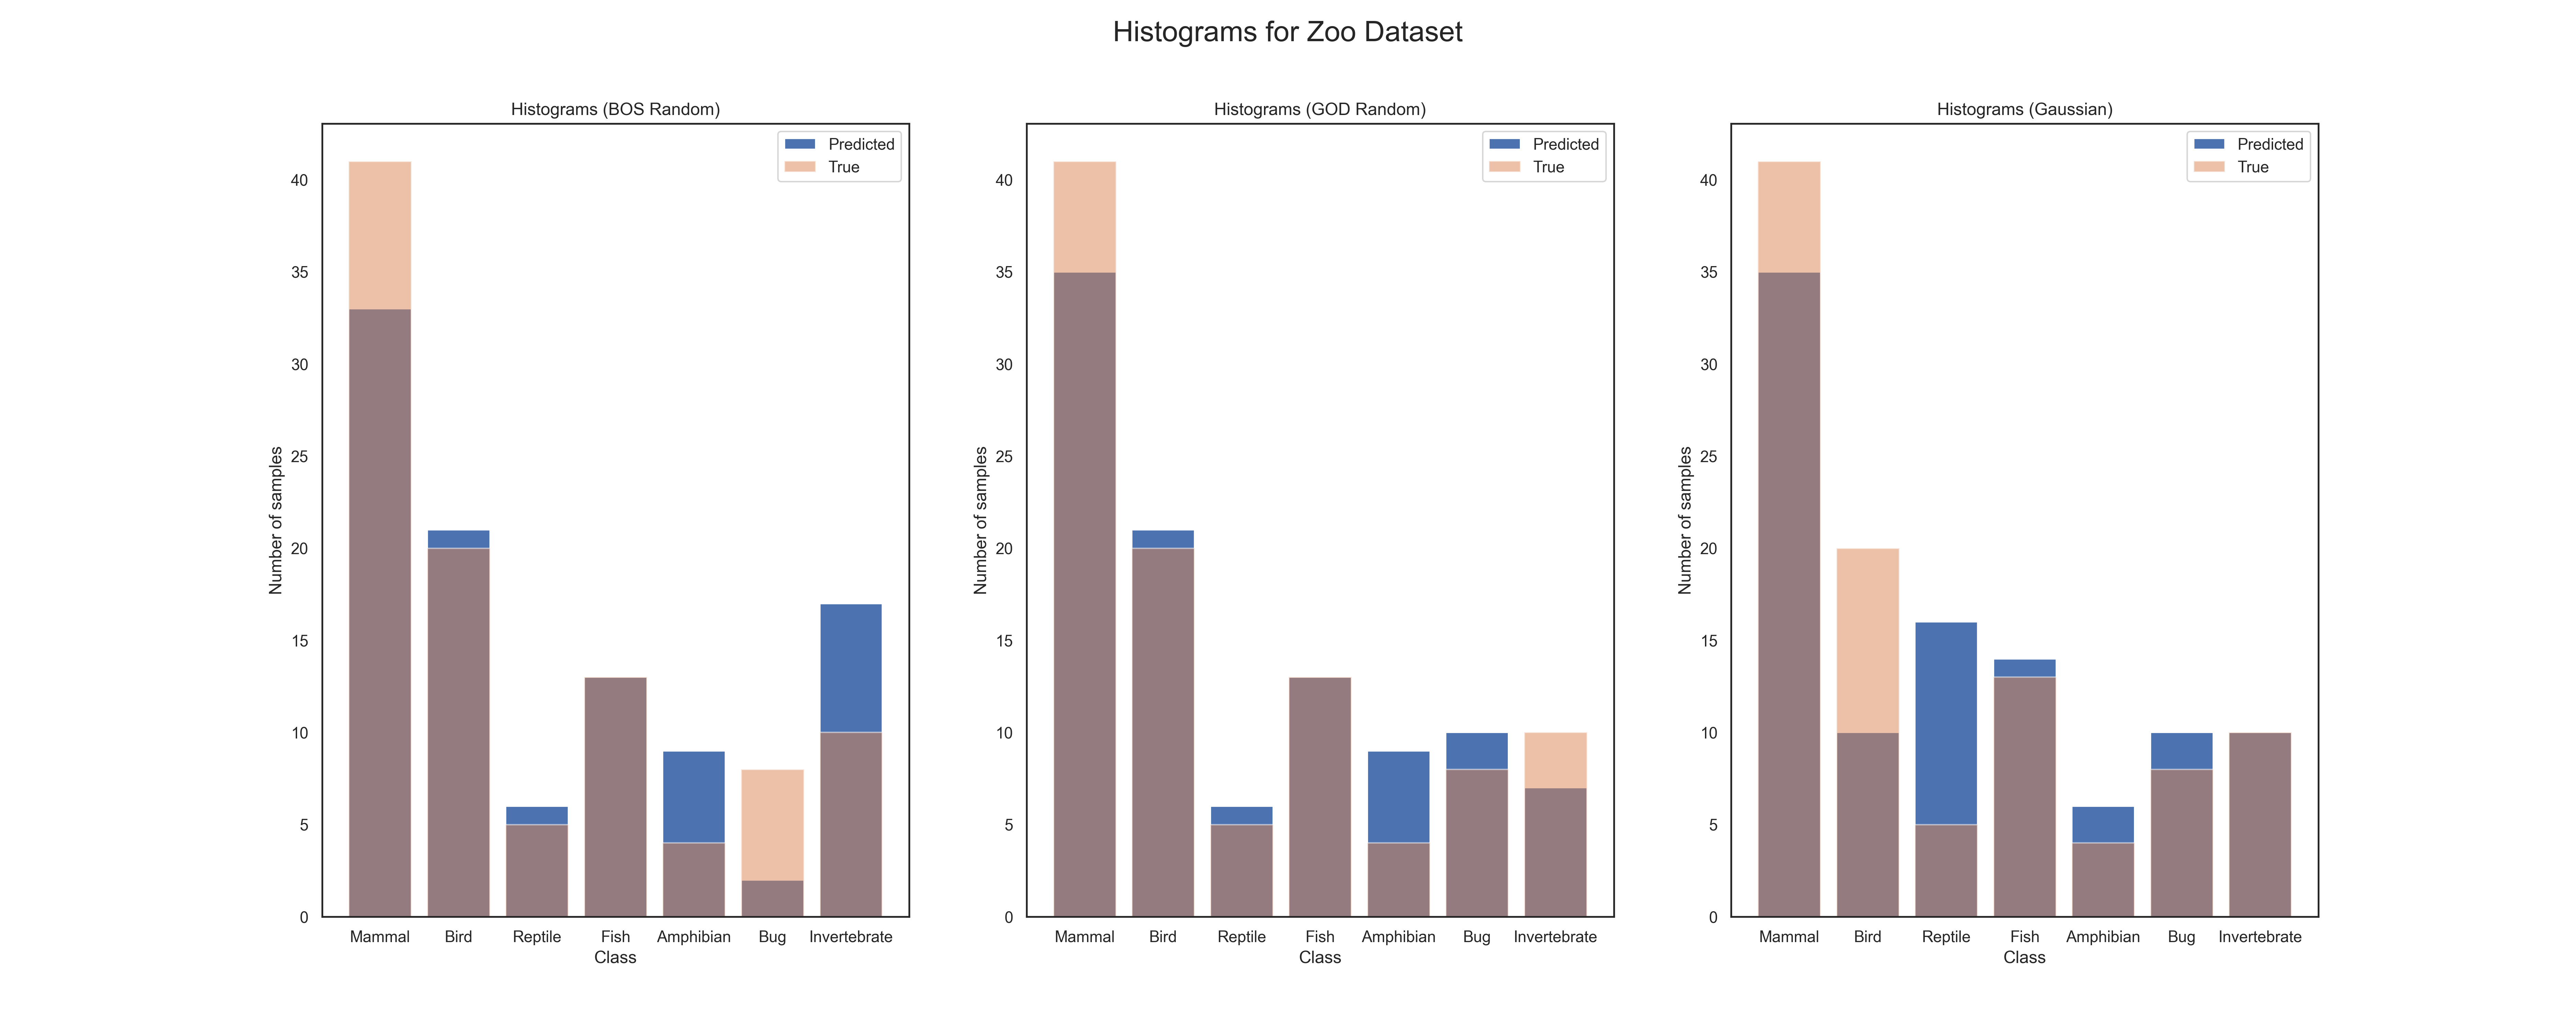
\includegraphics[width=\linewidth]{Attachments/histograms_zoo.png}
    \caption{Histograms for the Zoo dataset with different methods.}
    \label{fig:hist_zoo}
\end{figure}

\begin{figure}[H]
    \centering
    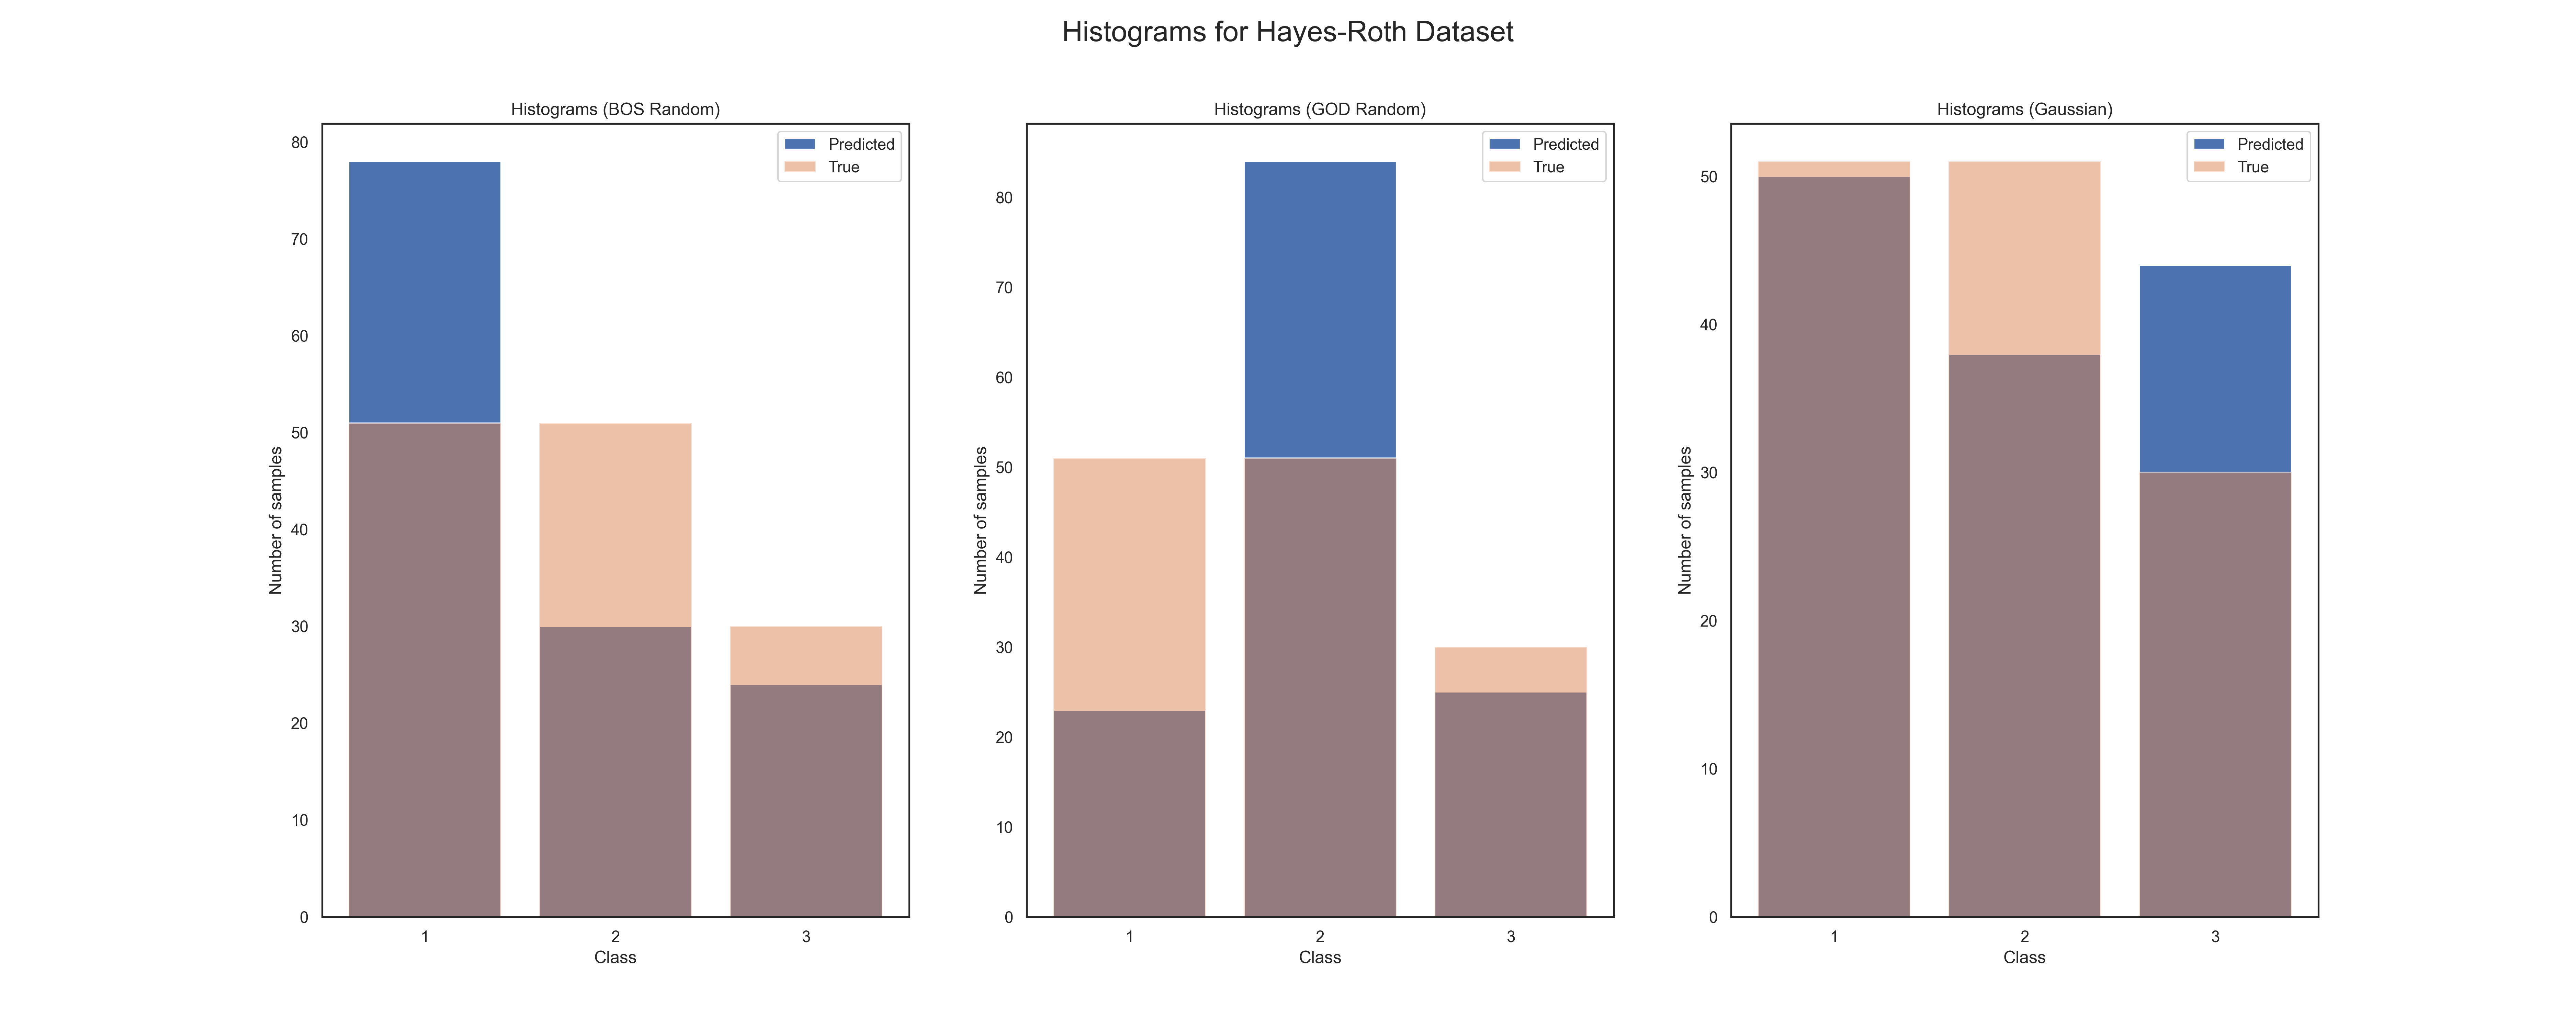
\includegraphics[width=\linewidth]{Attachments/histograms_hayes-roth.png}
    \caption{Histograms for the Hayes-Roth dataset with different methods.}
    \label{fig:hist_hr}
\end{figure}
